\documentclass[a4paper, 9pt]{article}

\usepackage{fullpage}
\usepackage{parskip}

\usepackage{authblk}

\usepackage{tikz}
\usepackage{graphicx}

\title{ARM Checkpoint}

\author{Ziming Feng}
\author{Zhan Shi}
\author{Zihao Zhao}
\author{Xinhe Wang}
\affil{Group 38}

\date{}

% Grabbed from https://www.overleaf.com/learn/latex/LaTeX_Graphics_using_TikZ%3A_A_Tutorial_for_Beginners_(Part_3)%E2%80%94Creating_Flowcharts
\usetikzlibrary{shapes.geometric, arrows}
% TikZ flowchart styles
\tikzstyle{startstop} = [rectangle, rounded corners, minimum width=3cm, minimum height=1cm, text centered, draw=black, fill=red!30]
\tikzstyle{io} = [trapezium, trapezium left angle=70, trapezium right angle=110, minimum width=3cm, minimum height=1cm, text centered, draw=black, fill=blue!30]
\tikzstyle{process} = [rectangle, minimum width=3cm, minimum height=1cm, text centered, text width=4cm, draw=black, fill=orange!30]
\tikzstyle{decision} = [diamond, minimum width=3cm, minimum height=1cm, text centered, draw=black, fill=green!30]
\tikzstyle{arrow} = [thick,->,>=stealth]

\begin{document}

\maketitle

\section{Group Organisation}

\subsection{Group Collaboration and Coordination}

Our group approached splitting the work for part 1 by engaging in brainstorming sessions to generate ideas for implementation,
and each member is responsible for the part they're most confident in. Ultimately, each person handled approximately equal workloads.

Regarding to tasks for each member, Ziming Feng produced data processing instructions execution and laid out the instruction struct,
Zhan Shi worked on decoding binary instructions and displaying the output,
Zihao Zhao dealt with execution for single data transfer and branch instructions, and Xinhe Wang worked on the overall emulator pipeline,
file handling and set up the Gitlab pipeline for building and testing.
Furthermore, all members contributed to debugging and optimising the code.

Our group would all be on campus on weekdays for the most efficient coordination, and we used WeChat (equivalent to WhatsApp) to communicate remotely.

\subsection{Reflection on Groupwork}

In our opinion, the group work exceeded the expectations, especially given that not all of us have experience in C programming or collaborative coding projects.
Communication was largely effective and constructive with everyone responding promptly,
although some members contributed less during brainstorming.
We agree that full participation in the initial planning discussions is essential so that every member understands the overall structure and goals before tackling individual tasks.
Going forward, we suggested that all members should attend and contribute to these sessions and make sure they are clear on our aims before coding begins.

Despite the challenge of producing substantial amounts of C code,, all members were able to complete their parts on time and with high quality,
while also actively engaging in debugging for their respective parts.

Nonetheless, we believe that establishing a standard for code style that everyone should follow before starting to code would prove helpful,
since we have spent considerable effort unifying the code style of each member when putting everything together in part 1,
and the process proved both time-consuming and error-prone.

\section{Implementation Strategies}

\subsection{Emulator Structure}

Our emulator consists of multiple modules and implements the execution pipeline suggested in the spec.
The storage module defines the representation for registers and memory, then groups them into the Storage struct,
which comprises registers and memory, and passes it to the execution phase via the initialisation function.
The instructions module contains the struct definitions for representing the binary instructions and the function to decode the 32-bit binary and organise it into our representations for the execution phase to use.
The design aim is to separate decoding from execution in the effort to reduce potential errors and simplify the debugging process.
The pipeline module handles the execution phase using the internal representations and implements the overall pipeline containing decoding.
Inside the module, the execution function comprises five helper functions, each handling a type of instruction.
Finally, all the helper functions used to achieve simple tasks common to all modules, such as accessing registers or memory and extracting bits from instructions, are grouped into the Utilities module.

Instead of using global variables for registers and memory, we chose to include the storage struct in function parameters.
The purpose of this design is that we can potentially use two copies of storage when working on part 2.
In our original conception, we would also be able to reuse the representations of instruction from part 1 in part 2. However, we have already completed part 2 as of this checkpoint, and it turned out to be troublesome,
so we ended up producing another intermediate representation for the assembler.
We are looking into how we might be able to merge these representations and eliminate the quite cumbersome structs.

\begin{figure}[h]
  \scalebox{0.5}{
    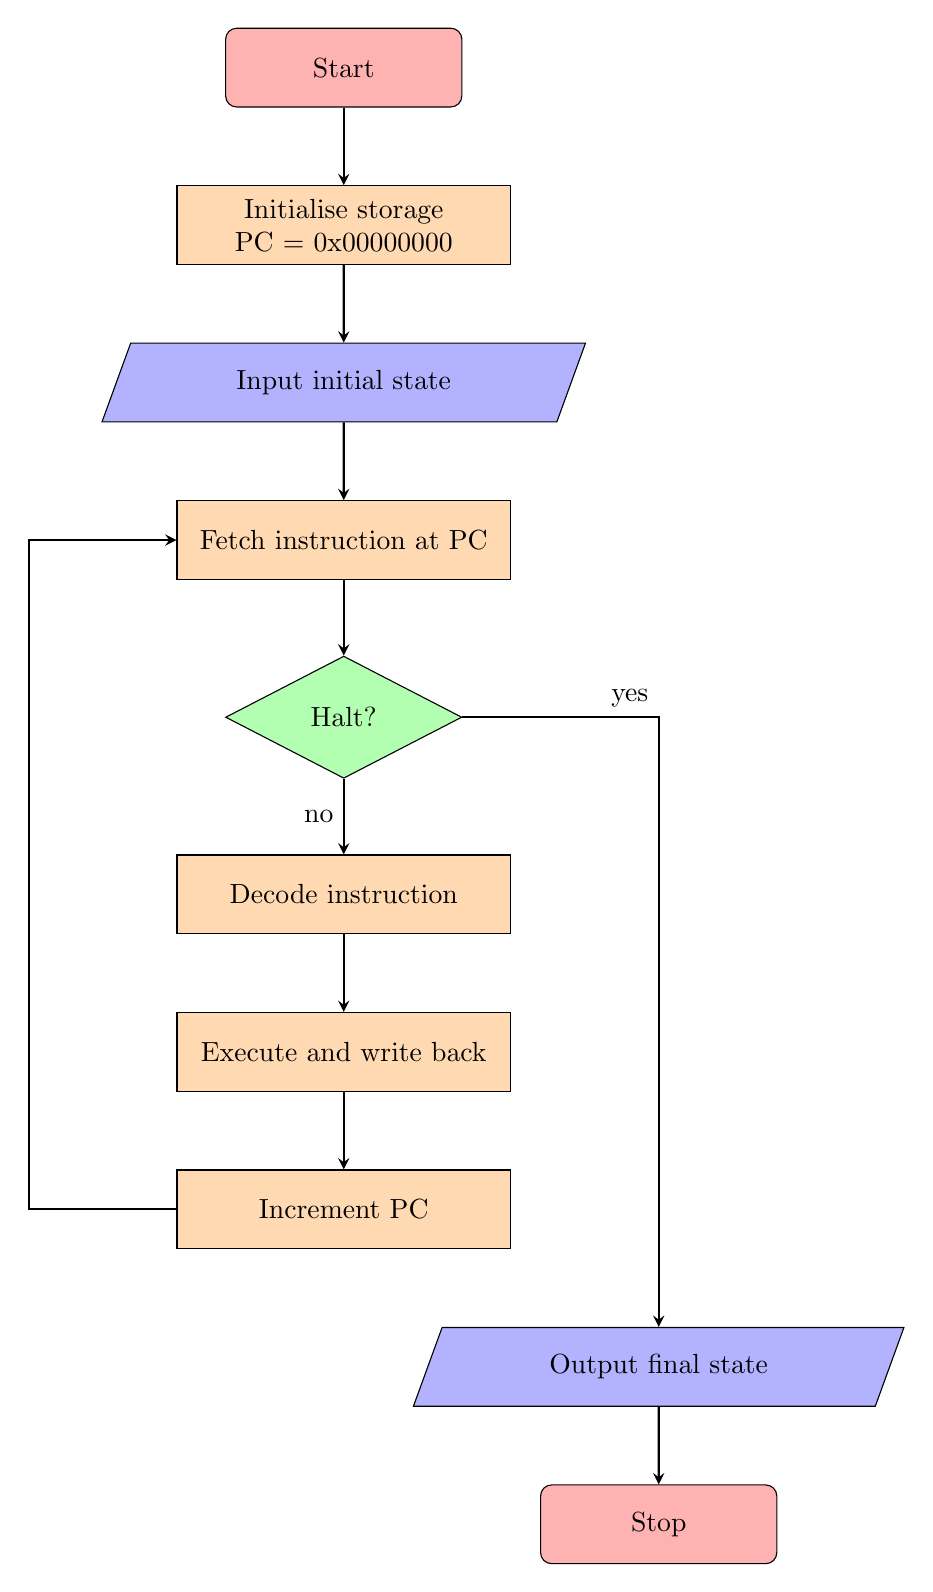
\begin{tikzpicture}[node distance=2cm]
      % Nodes
      \node (start) [startstop] {Start};
      \node (init) [process, below of=start] {Initialise storage PC = 0x00000000};
      \node (input) [io, below of=init] {Input initial state};
      \node (fetch) [process, below of=input] {Fetch instruction at PC};
      \node (halt) [decision, below of=fetch, yshift=-0.25cm] {Halt?};
      \node (decode) [process, below of=halt, yshift=-0.25cm] {Decode instruction};
      \node (execute) [process, below of=decode] {Execute and write back};
      \node (inc_pc) [process, below of=execute] {Increment PC};
      \node (output) [io, below of=inc_pc, xshift=4cm] {Output final state};
      \node (stop) [startstop, below of=output] {Stop};
      % Arrows
      \draw [arrow] (start) -- (init);
      \draw [arrow] (init) -- (input);
      \draw [arrow] (input) -- (fetch);
      \draw [arrow] (fetch) -- (halt);
      \draw [arrow] (halt) -- node[anchor=east] {no} (decode);
      \draw [arrow] (halt) -| node[anchor=south east] {yes} (output);
      \draw [arrow] (decode) -- (execute);
      \draw [arrow] (execute) -- (inc_pc);
      \draw [arrow] (inc_pc) -- ++(-4cm,0) |- (fetch);
      \draw [arrow] (output) -- (stop);
    \end{tikzpicture}
  }
  \centering
  \caption{Procedure of the emulator}
\end{figure}

\subsection{Challenging Parts in the Future}

When we finished part 1, we all agreed that the tokeniser and parser would be the most challenging tasks in part 2. 
Our solution was to use a union to group the operations with the same operands and binary representation into different structs in the intermediate representation,
so that the parser can identify the different patterns and organise the instructions.
This approach proved useful in the end.

Since some of us don't have experience working with Raspberry Pi, we expect part 3 to be somewhat challenging.
Hence, we are planning to watch some tutorials before we approach part 3.

We all agree that the extension would be the most difficult part as there are no guidelines to follow.
Having the extension based on Raspberry Pi would be more straightforward than software tools,
but we are also looking for inspiration from the Armv8 manual before landing on a final decision later.

\end{document}
